% Origen: sección "Apéndice" de Secciones/PI - Software.md
% Archivo apend5 por orden de creación; en template.tex va después de apend3.
\chapter{Complementos del software}
\label{C:ap-sw}

% Figuras de este apéndice + las compartidas.
\graphicspath{{figs/apendices/}{figs/comunes/}}

\section{Estructuras internas de \texorpdfstring{\texttt{libmca}}{libmca}}
\label{S:ap-sw-estructuras}

En la Tabla~\ref{t:ap-sw-estructuras} se nombran las estructuras internas de
\codigo{libmca}.

\begin{longtable}{|l|>{\raggedright\arraybackslash}p{0.39\textwidth}%
  |>{\raggedright\arraybackslash}p{0.30\textwidth}|}
\caption[Estructuras internas de \codigo{libmca}]{%
Resumen breve de las estructuras internas utilizadas en este
proyecto.\label{t:ap-sw-estructuras}} \\
\hline \encabezado \textbf{Bloque} & \textbf{Estructura} &
  \textbf{Funcionalidad} \\ \hline
\endfirsthead
\hline \encabezado \textbf{Bloque} & \textbf{Estructura} &
  \textbf{Funcionalidad} \\ \hline
\endhead
común & \codigo{mca\_bloque} & base de todo \emph{handle}: el bus y el último error \\ \hline
común & \codigo{mca\_reg\_t} & una fila del mapa de registros \\ \hline
común & \codigo{mca\_field\_t} & una fila de la tabla de campos \\ \hline
bus & \codigo{mca\_bus} & base de los \emph{backends} \\ \hline
bus & \codigo{mca\_bus\_vt} & las funciones de un \emph{backend} \\ \hline
bus & \codigo{devmem\_bus} & \emph{backend} de \codigo{/dev/mem} o de un fichero \\ \hline
bus & \codigo{cb\_bus} & \emph{backend} por \emph{callbacks} \\ \hline
bus & \codigo{mca\_bus\_ops} & las funciones que da quien abre por \emph{callbacks} \\ \hline
DDR & \codigo{mca\_mem} & la región de DDR del ring \\ \hline
MCA & \codigo{mca\_h} & \emph{handle}; guarda la geometría leída al abrir \\ \hline
MCA & \codigo{mca\_info\_t} & qué trae el \emph{bitstream} \\ \hline
MCA & \codigo{mca\_config\_t} & toda la configuración \\ \hline
MCA & \codigo{mca\_forma\_t} & una forma del banco de trapecios \\ \hline
MCA & \codigo{mca\_counters\_t} & contadores y tiempos \\ \hline
MCA & \codigo{mca\_last\_event\_t} & el último evento medido \\ \hline
TOP & \codigo{integration\_h} & \emph{handle}, sin estado propio \\ \hline
TOP & \codigo{integration\_info\_t} & versión y \emph{hash} del \emph{bitstream} \\ \hline
TOP & \codigo{integration\_modules\_t} & qué módulos trae \\ \hline
TOP & \codigo{integration\_slots\_t} & el \emph{slot} de cada módulo \\ \hline
TOP & \codigo{integration\_caps\_t} & la geometría publicada \\ \hline
TOP & \codigo{integration\_route\_t} & de dónde toma la señal un consumidor \\ \hline
TOP & \codigo{integration\_status\_t} & el PLL y el \emph{reset} del ADC \\ \hline
multitrigger & \codigo{multitrigger\_h} & \emph{handle}, sin estado propio \\ \hline
multitrigger & \codigo{multitrigger\_shield\_t} & el \codigo{trigger\_shield} \\ \hline
multitrigger & \codigo{multitrigger\_slope\_t} & el disparo por pendiente \\ \hline
multitrigger & \codigo{multitrigger\_pz\_t} & el disparo con polo-cero \\ \hline
multitrigger & \codigo{multitrigger\_status\_t} & el estado en vivo \\ \hline
osciloscopio & \codigo{osciloscope\_h} & \emph{handle}; guarda la geometría \\ \hline
osciloscopio & \codigo{osciloscope\_geometria\_t} & \codigo{RSZ}, \codigo{N\_CH}, \codigo{DW} y las aperturas \\ \hline
osciloscopio & \codigo{osciloscope\_calib\_t} & la calibración en la PL \\ \hline
osciloscopio & \codigo{osciloscope\_status\_t} & las FSM y los punteros \\ \hline
osciloscopio & \codigo{osciloscope\_adc\_cal\_t} & la calibración de librp, de la EEPROM \\ \hline
osciloscopio & \codigo{osc\_cal\_t} & esa calibración, lista para aplicar \\ \hline
lazo de la BRAM & \codigo{osciloscope\_lote\_cfg\_t} & la configuración de la corrida \\ \hline
lazo de la BRAM & \codigo{osciloscope\_lote\_estado\_t} & lo que sigue entre llamadas \\ \hline
lazo de la BRAM & \codigo{osciloscope\_lote\_t} & las columnas del lote donde escribe C \\ \hline
lazo de la BRAM & \codigo{osciloscope\_lote\_resultado\_t} & guardados y descartados; también la usa el ring \\ \hline
event\_ring & \codigo{osciloscope\_ring\_h} & \emph{handle}; guarda la DDR y un \emph{slot} \\ \hline
event\_ring & \codigo{osciloscope\_ring\_cfg\_t} & la configuración de la corrida \\ \hline
event\_ring & \codigo{osciloscope\_ring\_geometria\_t} & el \emph{slot} y el anillo, sin tocar el hardware \\ \hline
event\_ring & \codigo{osciloscope\_ring\_estado\_t} & lo que sigue entre llamadas \\ \hline
event\_ring & \codigo{osciloscope\_ring\_lote\_t} & las columnas del lote, más \codigo{ts\_hw} y \codigo{seq} \\ \hline
event\_ring & \codigo{osciloscope\_ring\_contadores\_t} & los contadores del hardware \\ \hline
event\_ring & \codigo{osciloscope\_ring\_medida\_t} & lo que acumula \codigo{medir} \\ \hline
generadores & \codigo{gen\_disparos\_cfg\_t} & los registros del motor de disparos \\ \hline
generadores & \codigo{gen\_estado\_t} & la cuenta y el estado de un generador \\ \hline
generadores & \codigo{gen\_pulsos\_h} & \emph{handle}; guarda el bus de HK \\ \hline
generadores & \codigo{gen\_pulsos\_cfg\_t} & toda la configuración de pulsos \\ \hline
\end{longtable}

\section{Detalle de los hilos de captura}
\label{S:ap-sw-hilos}

La Fig.~\ref{f:ap-sw-hilos-captura} es la Fig.~\ref{f:sw-flujo-sesion} con lo
que pasa adentro de cada hilo: las llamadas a C, quién tiene el GIL en cada
tramo, los mensajes a la PL por evento y el \ruta{.tmp} + \codigo{os.replace}
de cada archivo.

\begin{figure}[H]
\centering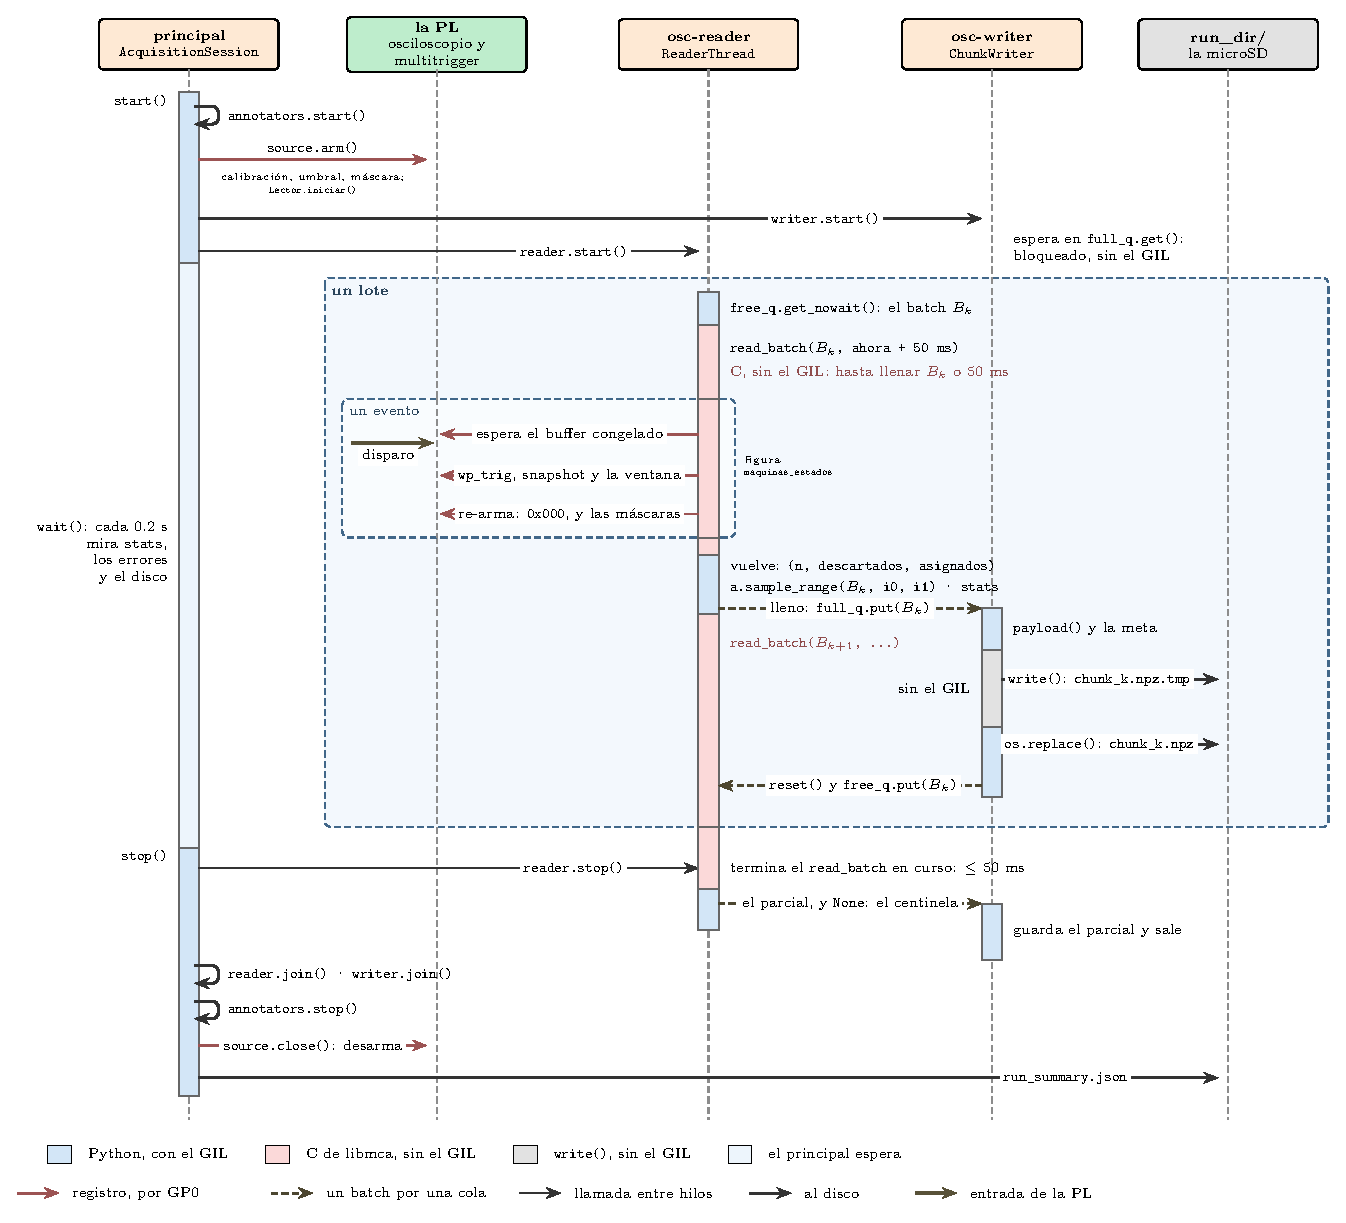
\includegraphics{apE_hilos_captura}
\caption[Detalle de los hilos de captura]{%
Una corrida con \codigo{BramSource}, de \codigo{start()} a \codigo{stop()}, sin
escala. El color sobre cada hilo dice qué corre y si tiene el GIL. El lector
pasa casi todo el tiempo en C (rojo, sin el GIL) y vuelve a Python (azul) una
vez por lote; el escritor pasa su tramo largo en el \codigo{write()} (gris,
también sin el GIL). Por eso no se frenan: el escritor guarda $B_k$ mientras el
lector ya llena $B_{k+1}$. Con \codigo{RingSource} el tramo de C es
\codigo{osciloscope\_ring\_\allowbreak leer\_lote} y los mensajes a la PL son los del ring;
el resto no cambia.\label{f:ap-sw-hilos-captura}}
\end{figure}

\section{Programación del \emph{bitstream}}
\label{S:ap-sw-bitstream}

La utilidad de línea de comandos por defecto de Pitaya simplemente cargaba un
nuevo \emph{bitstream}, independientemente de si este era incorrecto o de si el HW
presente estaba realizando una tarea antes de arrancar. Es así que expandimos la
función original de la carga con tres chequeos; su flujo de utilización se
presenta en la Fig.~\ref{f:ap-sw-bitstream}:
\begin{enumerate}
  \item Comprueba si la versión del Zynq es compatible con el \emph{bitstream}
    presente.
  \item Desactiva/activa las interconexiones AXI mediante puentes del OS.
  \item Implementa un \emph{watchdog} con el que comprueba que el sistema se mantiene
\end{enumerate}

\begin{figure}[H]
\centering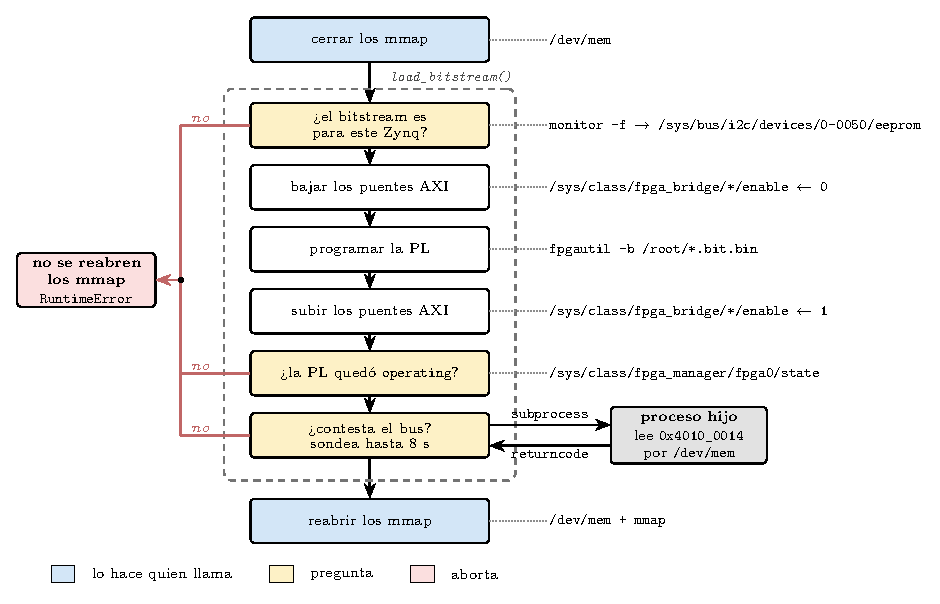
\includegraphics{apE_secuencia_bitstream}
\caption[Carga del \emph{bitstream}]{%
Metodología de la carga del \emph{bitstream} presente.\label{f:ap-sw-bitstream}}
\end{figure}

%%% Local Variables:
%%% mode: latex
%%% TeX-master: "template"
%%% End:
